\documentclass[a4paper,11pt]{article}
\usepackage[utf8]{inputenc}
\usepackage{graphicx}
\usepackage[spanish]{babel}


\begin{document}

\begin{titlepage}
\title{Ley de Ohm y teorema de Thevenin}
\author{Adrián Arce Sánchez}
\maketitle
\end{titlepage}

\begin{abstract}
En este informe se realiza el estudio del circuito de un entrenador mediante la ley de Ohm. Una vez estudiado se hará uso de este para probar el teorema de Thevenin.
\end{abstract}

\subsection*{Keywords}
Resistencia, Potenciómetro, Teorema de Thevenin, Entrenador, Polímetro.

\section{Introducción}
Muchas veces resulta difícil estudiar el circuito electrico interno de ciertos dispositivos debido a su complejidad o inaccesibilidad. En los casos en los que no se requiere de un gran detalle de lo que ocurre en su interior es posible simplificar su represetación a una fuente de tensión ideal conectada en serie a una resistencia. Esto es posible gracias al Teorema de Thevenin.

\section{Fundamento Teórico}
Uno de los conceptos clave a la hora de hablar de un circuito es la ley de Ohm. Esta, establece una relación de proporcionalidad entre la corriente que circula por un elemento circuital y la diferencia de potencial en los extremos del mismo. La constante de proporcionalidad que rige esta ley se denomina la esistencia. Se trata de una propiedad intrinseca de cada elemento circuital siendo la capacidad de oponerse al flujo de corriente que lo atraviesa. Esta propiedad depende de las dimensones del material con el que se ha construido dicho circuito.

\begin{displaymath}
V_{0}=RI
\end{displaymath}

Cuando por dos o más elementos circuitales fluye la misma corriente se dice que estos elementos están conectados en serie. En estos casos es posible crear un circuito equivalente en el cual todos los elementos que presentan resistencia a la corriente se representan mediante una unica resistencia cuyo valor queda definido como la suma de todas las resistencias de los elementos por separado.

\begin{displaymath}
R_{serie}=\sum_{i=1}^N R_{i}
\end{displaymath}

Además, podemos declarar a partir de las resistencias en serie, una asociación de resistencias. Capaces de repartir la tensión suminnistrada a cada uno de los ementos de la asociación. De este modo, la tensión "$V_i$" que el elemento i recibirá vendrá dado por la ecuación:

\begin{displaymath}
V_i=\frac{R_i}{\sum_{i=1}^N R_{i}}V_0
\end{displaymath}

\subsection{Teorema de Thevenin-Norton}
El teorema de Thevenin-Norton permite estudiar circuitos complejos a los cuales somos incapaces de acceder en su totalidad o resultan demasiado complejos para poder ser representados gráficamente.\\ \\
\begin{em}
“Cualquier red fuente resistiva lineal actúa desde una par de terminales como una fuente de tensión ideal, denominada tensión Thevenin, conectada en serie a una resistencia de valor RTh, denominada resistencia Thevenin”
\end{em}\\ \\
De este modo, es posible obtener la tensión Thevenin y la resistencia Thevenin en las siguientes condiciones:


\begin{displaymath}
V_{Th}=V_{ab}\|_{I=0}
\end{displaymath}

\begin{displaymath}
R_{Th}=R_{ab}\|_{Todas\,las\,fuentes\,cortocircuitadas}
\end{displaymath}

\newpage
\section{Realización de la Práctica}
En la primera parte de la sesión debiamos identificar los elementos circuitales que se encontraban en el entrenador. El circuito estaba compuesto por 4 resistencias, una conexión para un amperímetro, y una conexión para una fuente de ténsión variable.\\
En la siguiente tabla se muestran los valores obtenidos de las resistencias:\\

\begin{tabular}{|c|c|c|c|c|}
\hline 
/ & Valor nominal & Tolerancia & Valor medio & Precisión del polímetro \\ 
\hline 
R1 & 4,7 & 5\% & 4,656 & 0,045 \\ 
\hline 
R2 & 33 & 5\% & 33,11 & 0,33 \\ 
\hline 
R3 & 10,0 & 5\% & 9,97 & 0,12 \\ 
\hline 
R4 & 22,0 & 5\% & 21,79 & 0,23 \\ 
\hline 
\end{tabular}\\

Una vez obtenidos los valores de las resistencias, se montó el dibujo de la figura 2. En éste, se midió el valor de las tensiones Vab y Vbc en el intervalo de [0,20V] con estos datos que quedan reflejados en la tabla del apendice obtuvimos las siguientes gráficas:


\begin{figure}[hbtp]
\centering
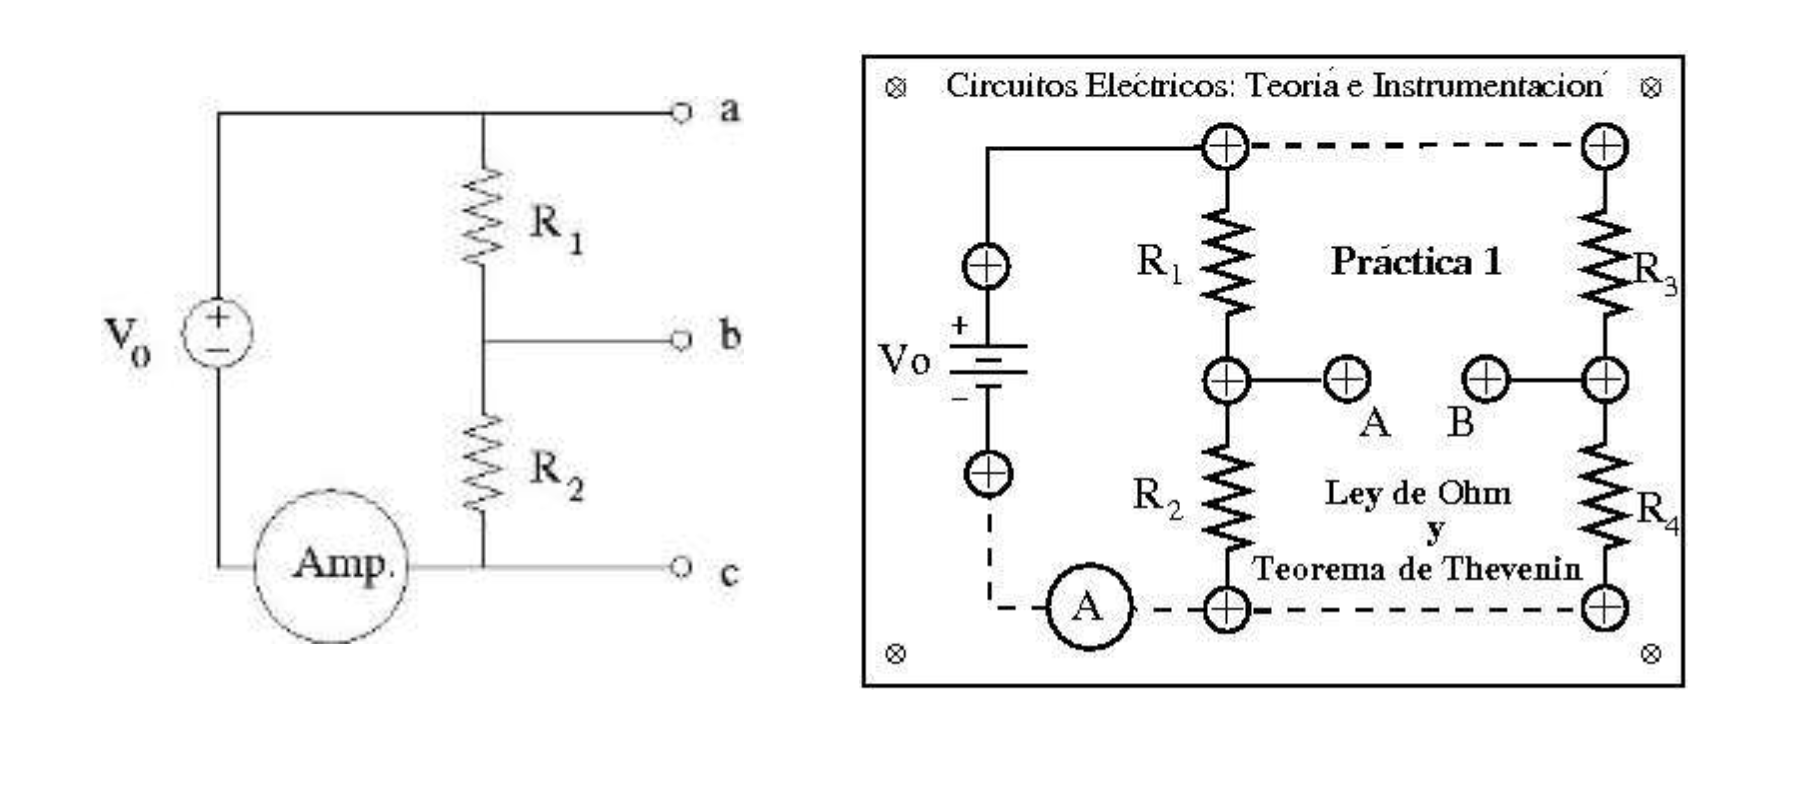
\includegraphics[scale=0.5]{Imagenes/Entrenador.png}
\caption{Circuito A del entrenador}
\end{figure}
\begin{figure}[hbtp]
\centering
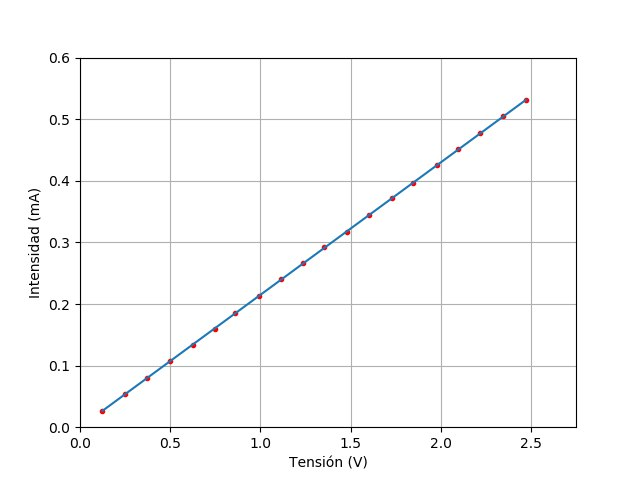
\includegraphics[scale=0.5]{Imagenes/Grafica_ac.jpg}
\caption{Gráfica ac}
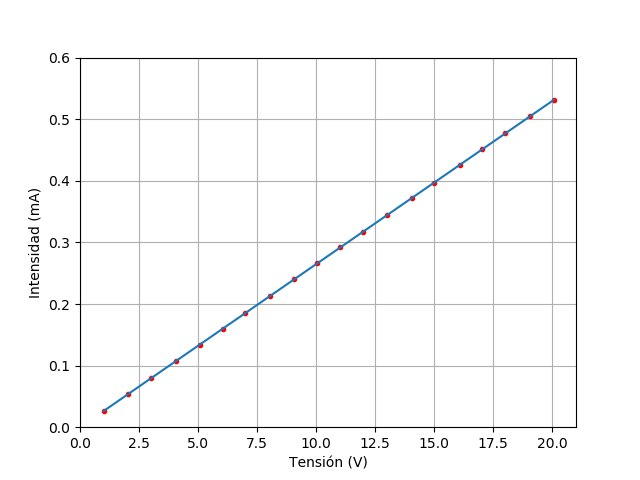
\includegraphics[scale=0.5]{Imagenes/Grafica_ab.jpg}
\caption{Gráfica ab}
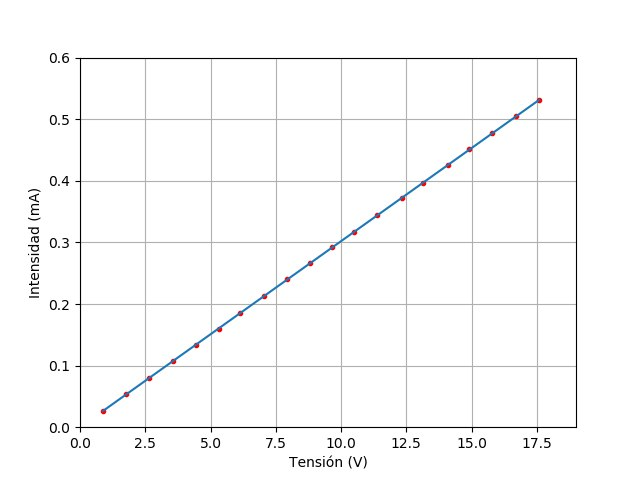
\includegraphics[scale=0.5]{Imagenes/Grafica_bc.jpg}
\caption{Gráfica bc}
\end{figure}

\newpage
\subsection{Theorema de Thevenin}

Para probar el teorema de thevenin se preparó en el entrenador el circuito de la figura 1 añadiendo dos cables de cobre.

\begin{figure}[hbtp]
\centering
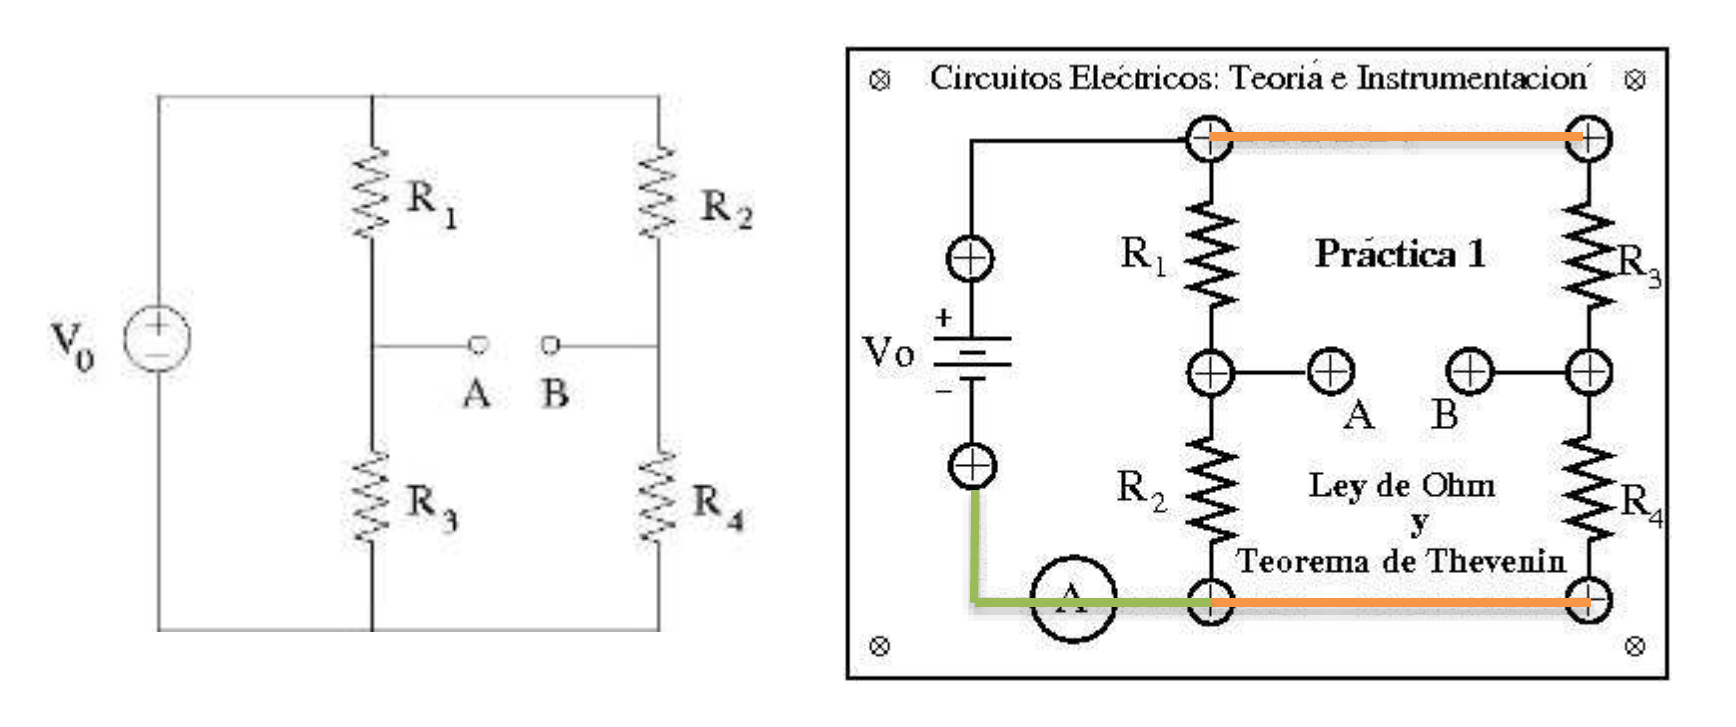
\includegraphics[scale=0.5]{Imagenes/Entrenador_B.png}
\caption{Circuito B del entrenador}
\end{figure}

Tras ello, procedimos a medir la tensión Thevenin y la resistencia Thevenin entre los terminales “A”, y “B”. Además se hizo uso de una resistencia de valor nominal de 100 $\Omega$ para medir la tensión en la resistencia cuando se conecta a los puntos “A”,y “B”. De este modo obtuvimos los siguientes resultados:\\

\begin{tabular}{|c|c|}
\hline
Tensión Thevenin experimental ($V_{Th}$) & 5,76 V\\
\hline
Resistencia Thevenin experimental ($R_{Th}$) & 10,92 k$\Omega$ \\
\hline
Valor de la resistencia de carga ($R_{carga}$) & 98,7 $\Omega$ \\
\hline
Tensión en la resistencia de carga ($V_{carga}$)	& 52,0 mV \\
\hline
\end{tabular}\\

Tras ello se montó un circuito equivalente formado por una fuente de tensión continua con valor $V_{Th}$ y un potenciómetro con una resistencia $R_{Th}$ tal y como aparece en la figura:

\begin{figure}[hbtp]
\centering
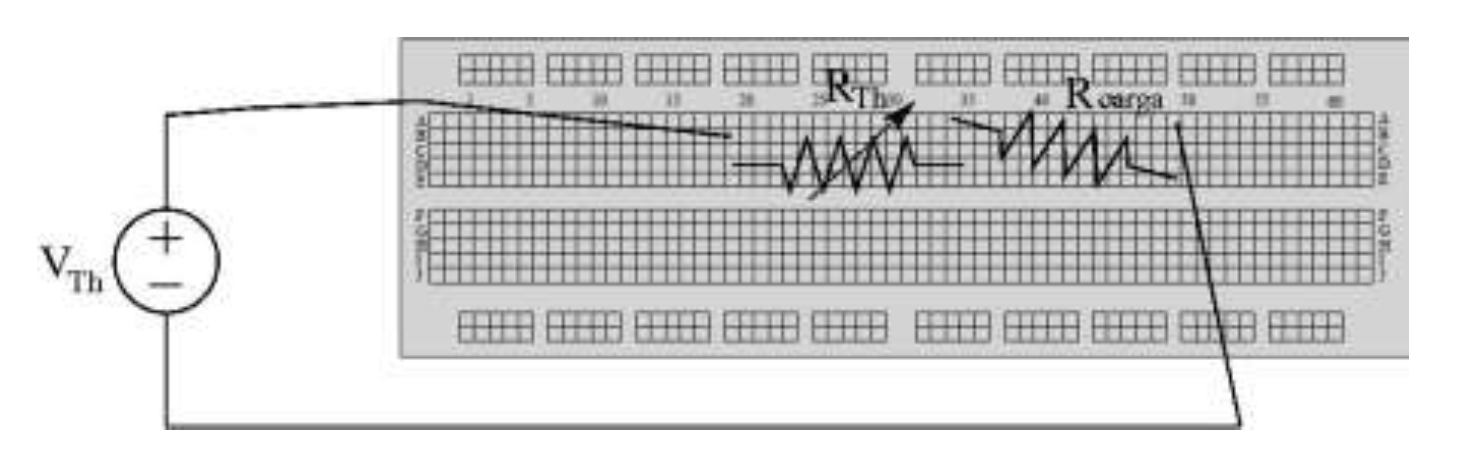
\includegraphics[scale=0.5]{Imagenes/circuito.png}
\caption{Circuito equivalente}
\end{figure}
Obteniendo un valor de 98,6 $\Omega$ y 51,6 mV. La diferencia de valores respecto al circuito original puede ser debido a o disponer de una fuente de tension de suficiente precision para alcanzar la tensión $V_{Th}$.

\newpage
\bibliography{Milibreria}
\bibliographystyle{plain} 

\nocite{Quintero2018}
\nocite{Zetina2000}

\section{Apéndice}
\subsection*{Datos del entrenador A}
\begin{tabular}{|c|c|c|c|}
\hline
$V$	&    $V_{ab}(V)$	  &      $V_{bc}(V)$	    &    $I(mA)$ \\
\hline
1,0	   & 	0,1232 $\pm$ 0,0008    &   0,877 $\pm$  0,006	 &   0,026 $\pm$  0,002\\
\hline
2,0	   &		0,2496 $\pm$ 0,0014    &   1,775 $\pm$  0,011	 &   0,054 $\pm$  0,003\\
\hline
3,0	   & 	0,372 $\pm$  0,0021    &   2,649 $\pm$  0,015	 &   0,08  $\pm$  0,003\\
\hline
4,0	   & 	0,5003 $\pm$ 0,0027    &   3,559 $\pm$  0,02	 &   0,107 $\pm$  0,003\\
\hline
5,0	   & 	0,6242 $\pm$ 0,0033    &   4,444 $\pm$  0,024	 &   0,134 $\pm$  0,003\\
\hline
6,0	   & 	0,748 $\pm$  0,006     &   5,322 $\pm$  0,029	 &   0,16  $\pm$  0,004\\
\hline
7,0	   & 	0,861 $\pm$  0,006     &   6,135 $\pm$  0,033	 &   0,185 $\pm$  0,004\\
\hline
8,0	   & 	0,992 $\pm$  0,007     &   7,06 $\pm$   0,06	 &   0,213 $\pm$  0,004\\
\hline
9,0	   & 	1,115 $\pm$  0,008     &   7,93  $\pm$  0,06	 &   0,24  $\pm$  0,004\\
\hline
10,0   & 	1,238 $\pm$  0,008     &   8,81  $\pm$  0,06	 &   0,266 $\pm$  0,005\\
\hline
11,0   & 	1,355 $\pm$  0,009     &   9,64  $\pm$  0,07	 &   0,292 $\pm$  0,005\\
\hline
12,0   & 	1,478 $\pm$  0,009     &   10,51 $\pm$  0,07	 &   0,317 $\pm$  0,005\\
\hline
13,0   & 	1,601 $\pm$  0,01	   &   11,39 $\pm$  0,08	 &   0,344 $\pm$  0,005\\
\hline
14,0   & 	1,732 $\pm$  0,011     &   12,32 $\pm$  0,08	 &   0,372 $\pm$  0,006\\
\hline
15,0   & 	1,848 $\pm$  0,011     &   13,15 $\pm$  0,09	 &   0,397 $\pm$  0,006\\
\hline
16,0   & 	1,982 $\pm$  0,012     &   14,1  $\pm$  0,09	 &   0,426 $\pm$  0,006\\
\hline
17,0   & 	2,097 $\pm$  0,012     &   14,92 $\pm$  0,09	 &   0,451 $\pm$  0,007\\
\hline
18,0   & 	2,219 $\pm$  0,013     &   15,79 $\pm$  0,1	 &   0,477 $\pm$  0,007\\
\hline
19,0   & 	2,348 $\pm$  0,014     &   16,71 $\pm$  0,1	 &   0,505 $\pm$  0,007\\
\hline
20,0   & 	2,473 $\pm$  0,014     &   17,59 $\pm$  0,11	 &   0,531 $\pm$  0,007\\
\hline
\end{tabular}
\end{document}